\section{Architectural Design}
\subsection{Overview}
We chose the three tier architecture for S\&C because we believe that it is a solid choice aligned with our goals and requirements.
The architecture is divided in three:
\begin{enumerate}
    \item\textbf{Presentation Tier}:
    This is essentially the user interface
    \item\textbf{Application Tier}:
    This layer is where the data are transformed and undergo a set of processes to make them available to the user interface
    \item\textbf{Data Tier}:
    This layer is where the data are stored and managed remotely.
\end{enumerate}
This is the visualization of the 3-tier logic. \cite{3Tier}\\
\begin{figure}[h!]
        \centering  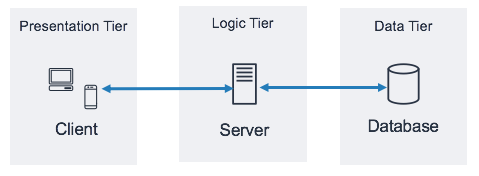
\includegraphics[width=1\textwidth]{DD/Images/aws.png}
        \label{fig:3Tier}
\end{figure}
\\
We also chose to use REST APIs to make the presentation layer and application layer communicate.  \\
The following image displays how an API works\cite{REST}:
\begin{figure}[h!]
        \centering  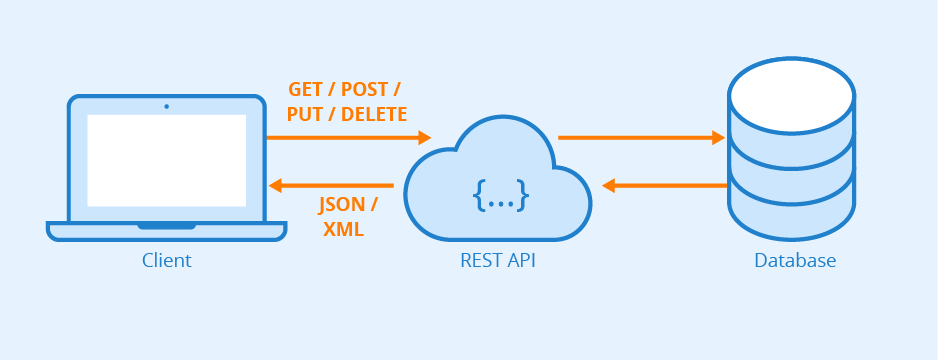
\includegraphics[width=1\textwidth]{DD/Images/rest.png}
        \label{fig:RESTAPI}
\end{figure}
\newpage
\subsection{Component View}
This section aims to give a general representation of the core components of the system and how they interact together without focusing on the internal details.
Indeed it is important to grasp the division in modules and the interactions among them. In the component view image it is clearly distinguishable the 3-tier architecture and composed by the WebApp, the Back-End composed by all the modules depicted and listed below and the Database. Since all the logic is implemented in the middle layer, namely the S\&C Server, that is where all the modules are and interact.
The main components of the back-end are:
\begin{enumerate}
    \item \textbf{WebApp}: it is the component in charge of providing the user interface for interacting with the system. It relies on the API to fetch and send data for various operations.
    \item \textbf{S\%C Server}
    \begin{itemize}
        \item \textbf{SearchManager}: it is the component in charge of receiving and handling the search requests about the internship positions issued by the students 
        \item \textbf{RegistrationManager}: it is the component in charge of managing the registration of the users.
        \item \textbf{LoginManager}: it is the component in charge of the login of the users
        \item \textbf{NotificationManager}: it is the component in charge of sending the notifications to users, including push notifications and confirmation emails used to validate email accounts in the registration process
        \item \textbf{ProfileManager}: it is the component in charge of handling user profile information. It is supposed dot interact with all the other components in order to keep the profile of the user up to date.
        \item \textbf{InternshipManager}: it is the component in charge of managing the internships. It manages the internship status, the communication, the assessment process (if needed), publishing of news related to the internships.
        \item \textbf{ApplicationManager}: it is the component in charge of keeping track of the status application and its details.
        \item \textbf{API}: it is the component that allows the back-end to interact with the requests from the front-end.
    \end{itemize}
    \item \textbf{Database}: it is the component in charge of storing all the information relevant to the platform.


\end{enumerate}
\newpage
\begin{figure}[h!]
        \centering  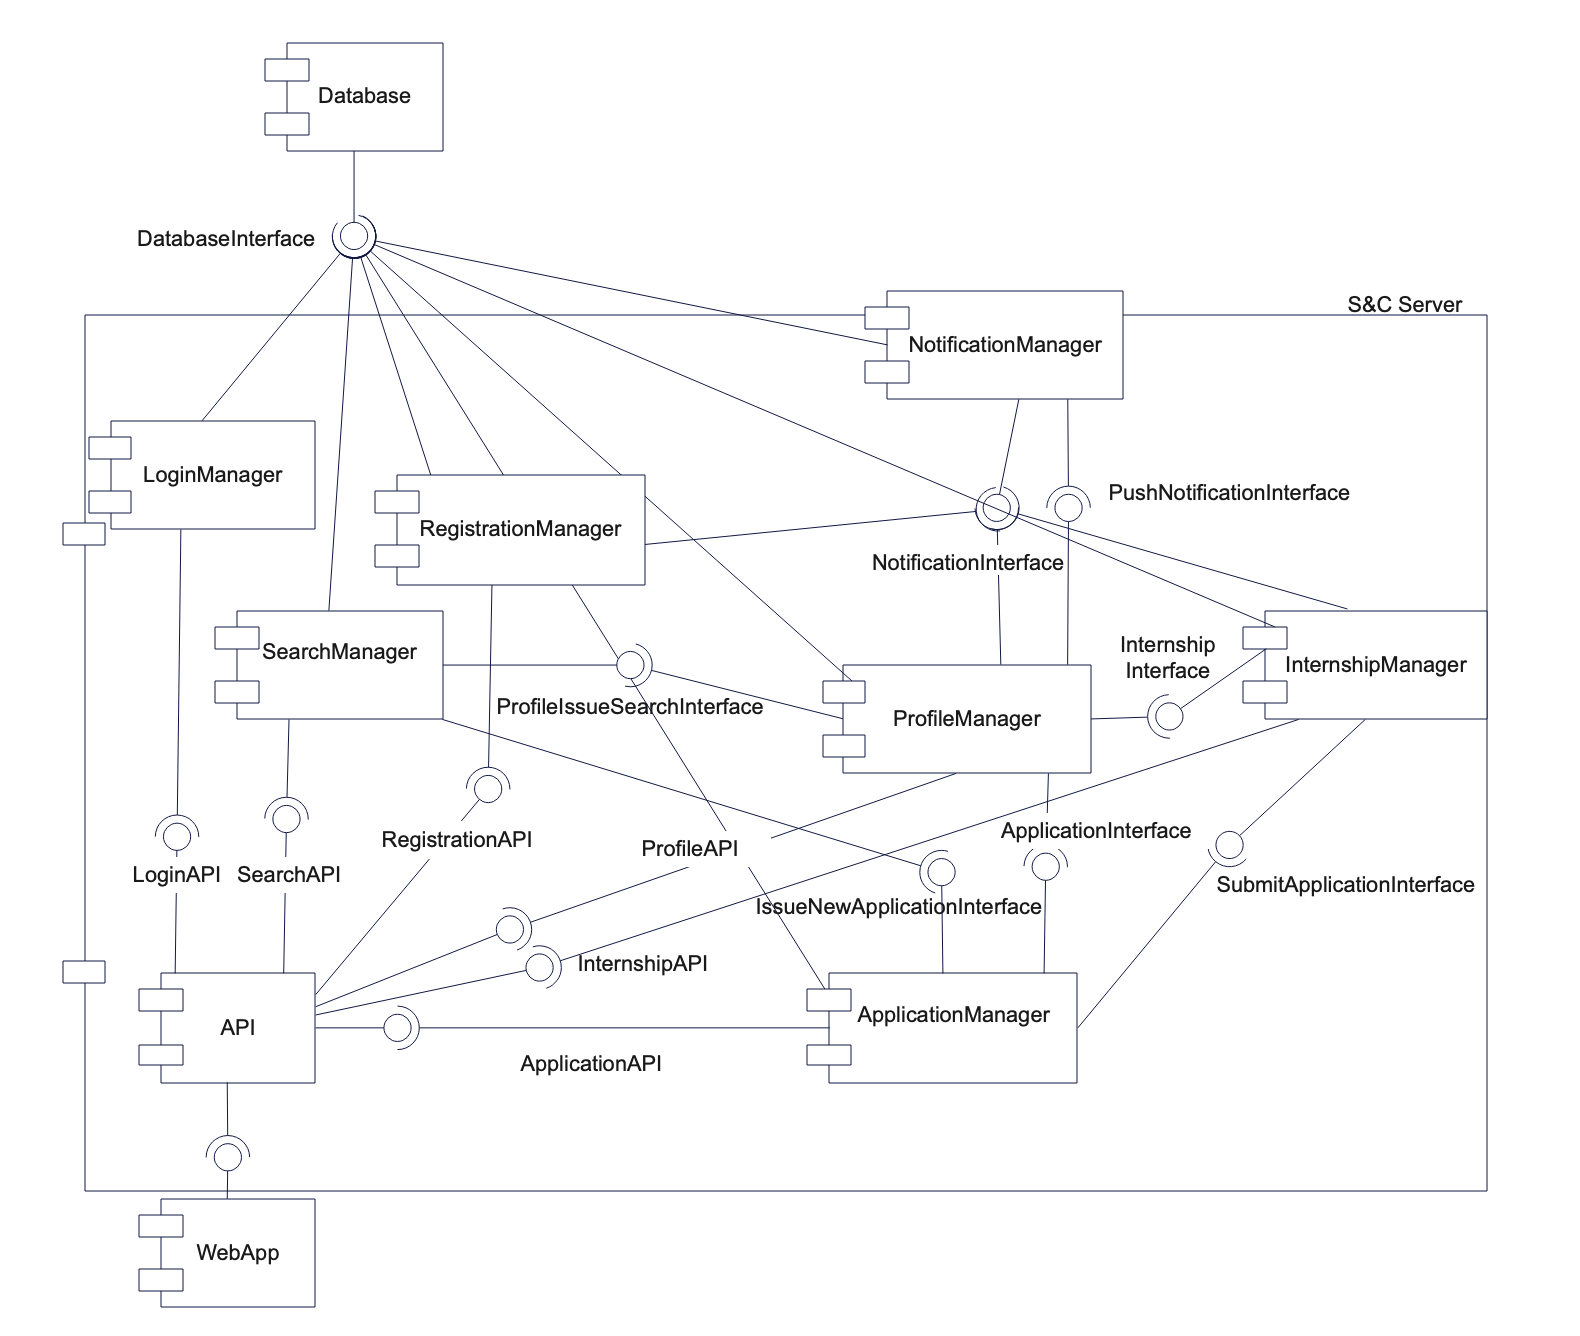
\includegraphics[width=1\textwidth]{DD/Images/CD.png}
        \label{fig:ComponentViewDiagram}
\end{figure}
\newpage

\subsection{Selected Architectural Styles and Patterns}
\subsubsection{3-Tier Architecture}
As already mentioned in the overview above, the decision to go for the 3-tier architecture is based on the belief that this type of architecture is well suited to the kind of application that it is going to be developed.
The first immediate benefit comes from the modularization which is the key feature of this type of architecture and from which indeed its name derives. The 3 independent layers are: 
\begin{itemize}
    \item \textbf{Presentation layer}: this corresponds to the front-end which is composed by the web pages and web interfaces with which the users interact.
    \item \textbf{Application layer}: this corresponds to the back-end which is where the logic of the application resides. 
    \item \textbf{Data layer}: this corresponds to the database which is the place where data are stored permanently.
\end{itemize}
The choice of implementing a three-tier architecture has several advantages.
\begin{itemize}
    \item The various tiers can be developed simultaneously and independently by different people or teams of people making the development phase faster
    \item The division in three tiers makes the separation of different functions more clear and makes the code easier to be understood and maintained
    \item The separation in three allows each layer to be scaled independently from the others, thus enhancing the overall scalability of the web application
\end{itemize}
To facilitate the communication between the presentation  and the application layers we decided to adopt the use of REST APIs. This choice brings many advantages:
\begin{itemize}
    \item \textbf{Decoupling}: it allows the developers to separate the scope and the concerns of the modules in three different layers, making the maintenance of the web application and the deployment of new features easier.
    \item \textbf{Easier future integration with third party services}: if for any reason in the future it will be necessary to add third party services they could be  effortlessly integrated into the system. 
    \item \textbf{Standard formats of communication}: REST APIs use standard HTTP methods and the JSON format to communicate which are the common standard for the world wide web.
    \item \textbf{Scalability}: each tier can be scaled independently from the others (up to a certain point of course).
\end{itemize}

\newpage
\section{Runtime View}

\begin{enumerate}
    
    \item User Login
    \begin{figure}[h!]
            \centering  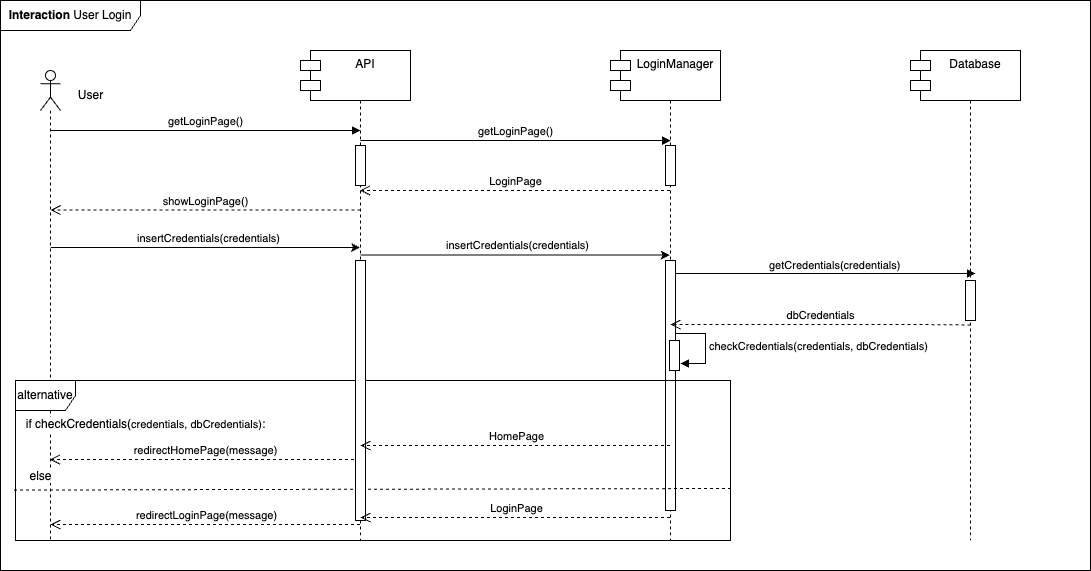
\includegraphics[width=1\textwidth]{DD/Images/Interactions/INT01_UserLogin.drawio.png}
            \label{fig:ComponentViewDiagram}
    \end{figure}
    
    \newpage
    \item User Logout
    \begin{figure}[h!]
            \centering  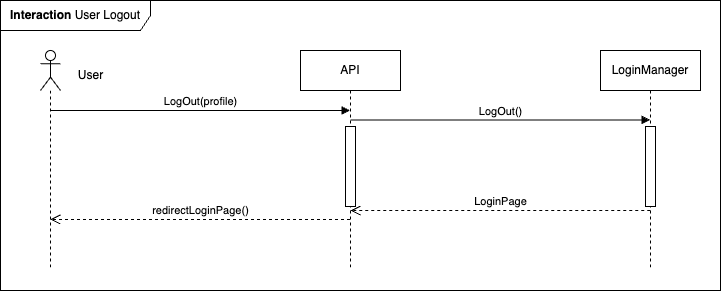
\includegraphics[width=1\textwidth]{DD/Images/Interactions/INT02_UserLogout.drawio.png}
            \label{fig:ComponentViewDiagram}
    \end{figure}

    \newpage
    \item User Update
    \begin{figure}[h!]
            \centering  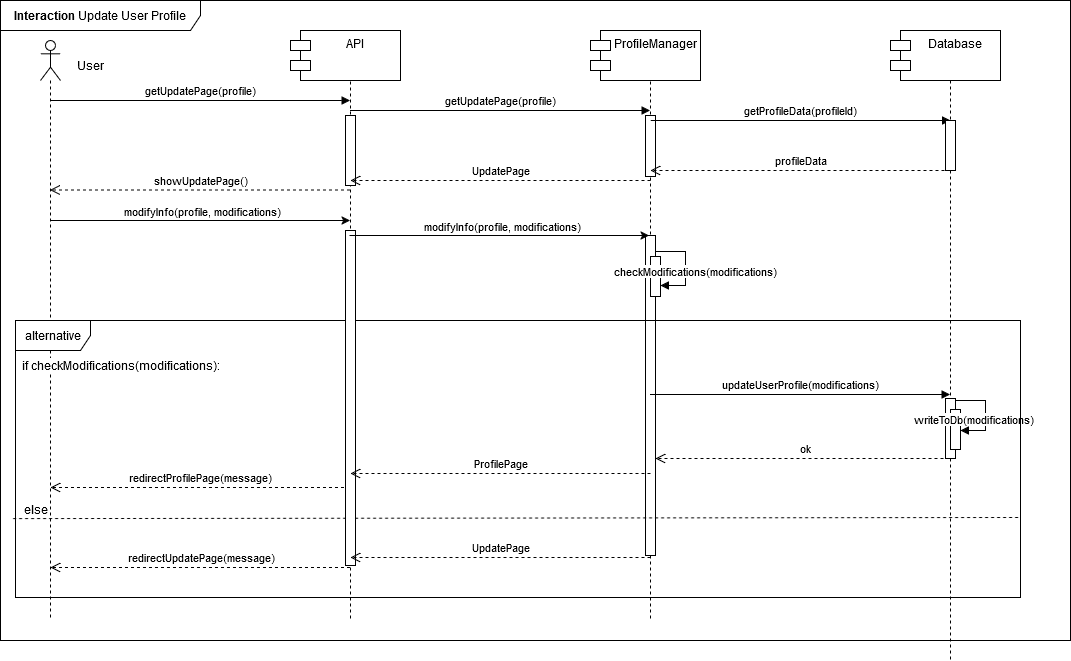
\includegraphics[width=1\textwidth]{DD/Images/Interactions/INT03_UserUpdate.drawio.png}
            \label{fig:ComponentViewDiagram}
    \end{figure}

    \newpage
    \item Student Registration
    \begin{figure}[h!]
            \centering  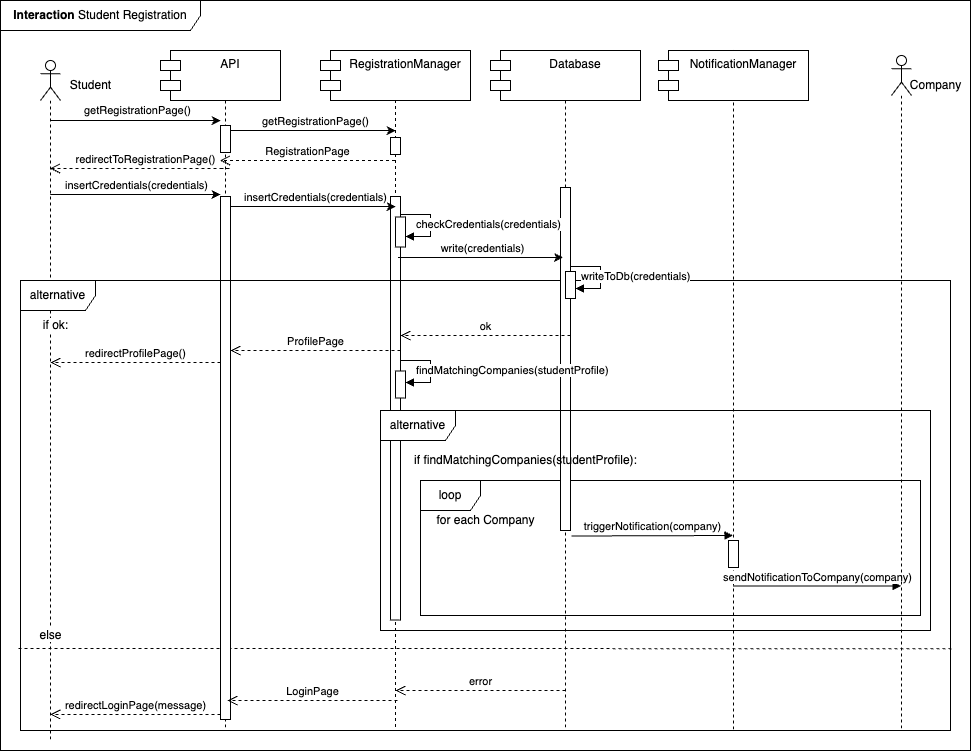
\includegraphics[width=1\textwidth]{DD/Images/Interactions/INT04_StudentRegistration.drawio.png}
            \label{fig:ComponentViewDiagram}
    \end{figure}

    \newpage
    \item Internship Search
    \begin{figure}[h!]
            \centering  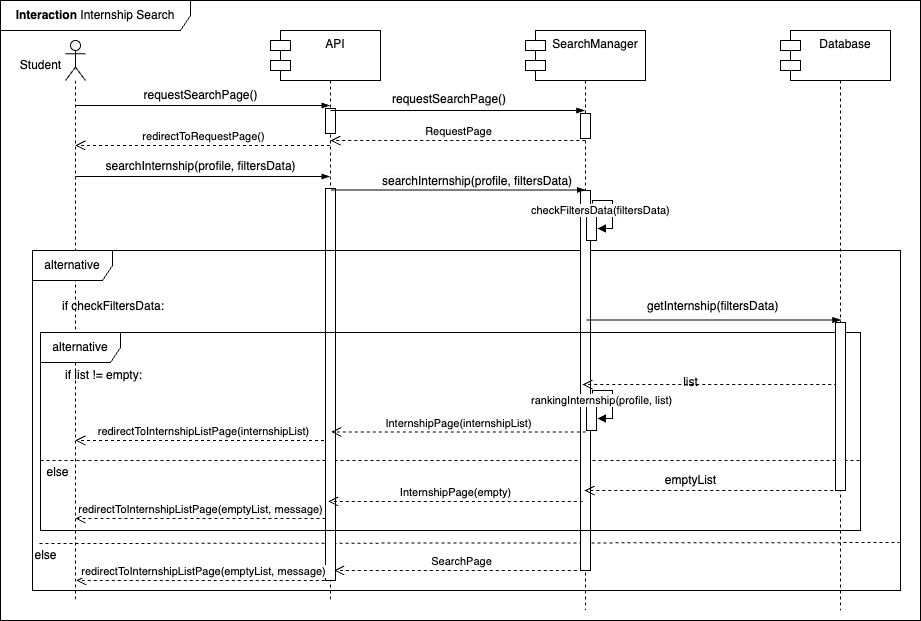
\includegraphics[width=1\textwidth]{DD/Images/Interactions/INT05_InternshipSearch.drawio.png}
            \label{fig:ComponentViewDiagram}
    \end{figure}
    
\end{enumerate}